\begin{align*}
    \polynomialP{1}{X}{0} &= 0 \\
    \polynomialP{1}{X}{1} &= 6X - 5 \\
    \polynomialP{1}{X}{2} &= 18X - 28 \\
    \polynomialP{1}{X}{3} &= 36X - 81 \\
    \polynomialP{1}{X}{4} &= 60X - 176 \\
    \polynomialP{1}{X}{5} &= 90X - 325 \\
    \polynomialP{1}{X}{6} &= 126X - 540 \\
    \polynomialP{1}{X}{7} &= 168X - 833 \\
    \polynomialP{1}{X}{8} &= 216X - 1216 \\
    \polynomialP{1}{X}{9} &= 270X - 1701 \\
    \polynomialP{1}{X}{10} &= 330X - 2300 \\
    \polynomialP{1}{X}{11} &= 396X - 3025 \\
    \polynomialP{1}{X}{12} &= 468X - 3888 \\
    \polynomialP{1}{X}{13} &= 546X - 4901 \\
    \polynomialP{1}{X}{14} &= 630X - 6076 \\
    \polynomialP{1}{X}{15} &= 720X - 7425 \\
    \polynomialP{1}{X}{16} &= 816X - 8960 \\
    \polynomialP{1}{X}{17} &= 918X - 10693 \\
    \polynomialP{1}{X}{18} &= 1026X - 12636 \\
    \polynomialP{1}{X}{19} &= 1140X - 14801 \\
    \polynomialP{1}{X}{20} &= 1260X - 17200
\end{align*}
\begin{figure}[H]
    \centering
    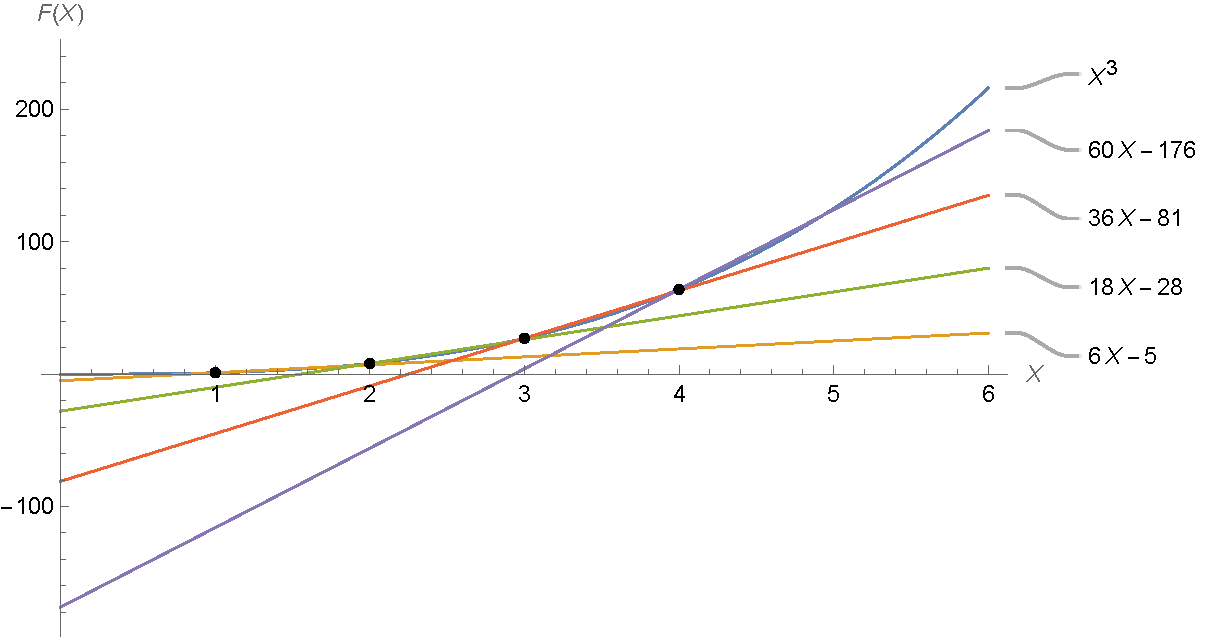
\includegraphics[width=1\textwidth]{sections/images/01_plots_cubes_with_p1}
    ~\caption{Polynomials $P(1, X, N)$ for N=1..4}\label{fig:figure}
\end{figure}
Intervals of convergence:
\begin{itemize}
    \item $6X - 5$: $1 \leq X \leq 1$ with $E \leq 0\%$
    \item $18X - 28$: $2 \leq X \leq 3$ with $E \leq 10\%$
    \item $36X - 81$: $2.9 \leq X \leq 4.1$ with $E \leq 5\%$
    \item $60X - 176$: $3.9 \leq X \leq 5.3$ with $E \leq 5\%$
\end{itemize}
